%! program = pdflatex

%\documentclass[12pt,a4paper]{memoir} % for a long document
\documentclass[10pt,letter,final,article,twocolumn]{article} % for a short document
\usepackage[left=0.25in,top=0.25in,right=0.25in,bottom=0.25in,nohead,nofoot]{geometry} 
\usepackage{titling,url}
\usepackage{graphicx}
% See the ``Memoir customise'' template for some common customisations
% Don't forget to read the Memoir manual: memman.pdf

\newcommand{\rpc}[1]{\emph{#1}}

\title{LWMR: Lightweight MapReduce}
\author{Athula Balachandran \\
{\tt abalacha@cs.cmu.edu}
\and
Wolfgang Richter \\
{\tt wolf@cs.cmu.edu}
\and
Erik Zawadzki \\
{\tt epz@cs.cmu.edu}}
\date{February 12, 2010} % delete this line to display the current date

%%% BEGIN DOCUMENT
\begin{document}

\pagestyle{empty}
\maketitle
\thispagestyle{empty}

\section{Problem Definition}
MapReduce~\cite{mapreduce08} is a framework that allows programmers to easily write applications that process large data-sets in a reliable and fault-tolerant manner on large clusters involving commodity hardware. The basic implementation  comprises of two stages---map and reduce. The input data set is split into independent chunks and are parallely processed by the map tasks. The output from this stage is then passed (sometimes after an intermediate local sorting stage called combine) to the reduce tasks. The framework abstracts all details like scheduling tasks, monitoring them and re-execution of failed tasks. 

The architecture typically conisists of a master node and several worker nodes that store data as well as do map/reduce jobs assigned by the master. The fact that the worker nodes store data as well as process them has been used to come up with efficient scheduling techniques that take into account locality and minimization of network traffic.

Most of the already existing implementations of MapReduce try to minimize communication overhead between the worker machines. However memory footprint is not of important consideration in many design decisions. This is of importance while designing MapReduce for systems like FAWN~\cite{fawn09}. In this project, we try to identify design possibilities that are key to decreasing memory footprint and we plan to reimplement a light weight MapReduce architecture that can be potentially be used by systems like FAWN.

\section{Previous Work}

As a foundation, we are designing our implementation based on the original 
description of MapReduce~\cite{mapreduce08}.  Other systems such as
Dryad~\cite{dryad07} provide design considerations and expose areas
where we can innovate with our implementation.  Our implementation on top
of FAWN~\cite{fawn09} introduces a particular constraint that the original
MapReduce design did not consider: low memory.  In addition, FAWN uses
flash storage as its principal storage medium which introduces another
area for MapReduce research---the original MapReduce design assumes a
storage medium of hard drives.  

Several other competing MapReduce implementations, such as
Disco~\cite{disco10}, Hadoop~\cite{hadoop10}, Sector and
Sphere~\cite{sphere09}, offer more examples to draw from for design
decisions.  Research has also shown that techniques such as merging the
MapReduce stages~\cite{barrier10}, and dynamically prioritizing resource
usage~\cite{sandholm09} offer substantial performance benefits over the
standard MapReduce design---techniques which have only been simulated
before.  Finally, we can take advantage of FAWN's energy efficiency which is
an active area of research with MapReduce as reflected in
Gordon~\cite{gordon09},  and work analyzing MapReduce traces for future
energy efficiency goals~\cite{chen10}.

\section{Architecture}



\begin{figure}[htbp]
\begin{center}
\resizebox{0.9\columnwidth}{!}{
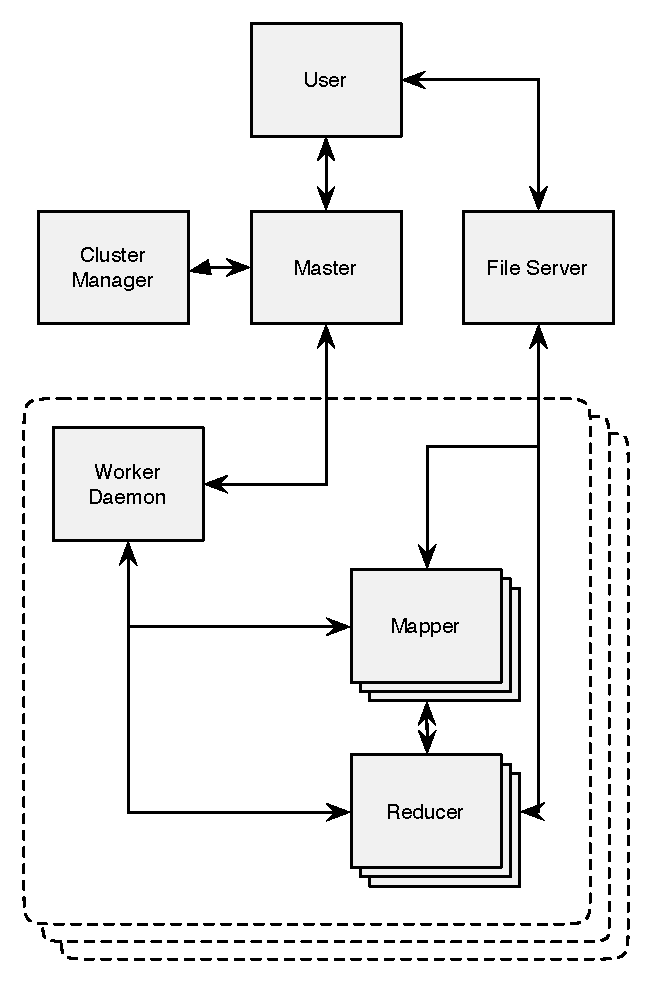
\includegraphics{Architecture.pdf}
}
\caption{A diagram of the major components of our architecture.}
\label{fig:arch}
\end{center}
\end{figure}


Our proposed architecture is shown in Figure~\ref{fig:arch}. This design is largely the same as the one presented in 
%\citet{dean04mapreduce}
?, with some additional detail. In particular, we have a worker daemon on each worker node that mediates communication between the master and the worker threads. We will explain the architecture by taking the reader through a typical MapReduce job.

\subsection{Typical Use}

The user contacts a master process and submits the MapReduce job using the \rpc{SubmitJob} RPC call, which the user will wait on (indeed, this is the only synchronous RPC call  that we will use). In the initial version of our system we will assume that there is a single well-known master that is always available (fails of the master are catastrophic). The user programs to carry out the Map and Reduce operations. Right now we are planning for these to be precompiled executables that are located on the DFS.

The master job then requests that the worker daemon on each node starts one or more mappers with \rpc{StartMapper}. The master will try to place mapper jobs on nodes that have a replicated copy of the appropriate input split.

We are assuming in this phase of the work that the user has access to the complete cluster and that the current MapReduce job is the only job running on the system. Later iterations of our work will have to include interactions with a cluster resource manager.

 The worker daemon, upon receipt of a mapper work request, spawns a new mapper thread for each request it gets. Because the worker daemon delays or rejects work requests the master is completely responsible for work scheduling. The  \rpc{StartMapper} call includes a list of input chunks from the DFS. For now, we will assume that each chunk belongs to a single file and that we do not have to worry about the boundaries of multi-chunk files---\textit{e.g.} if a text document spans two chucks a word does not start in one block and end in another.

The mapper thread buffers and writes the intermediate key-value pairs to local disk. Upon competition of the job, the mapper informs the worker daemon with \rpc{ReportLocalWorkComplete}, and exits. The worker daemon then contacts the master with \rpc{ReportWorkComplete} to inform it that it has some complete work.

In response to this new work the master may creates some new reducers with \rpc{StartReducer}. If all the necessary reducers exist, the master informs the existing workers that they have some new work with \rpc{ReportNewWork}. If the intermediate key/values  are local, then the reducer can read them right from disk. If not, then the key/values are requested from the remote worker daemon with the \rpc{SendDate} call. All of the intermediate data is read before the reducer starts executing the user's code.

At this point the reducer thread runs the user's code and writes a temporary local file with the output. Upon completion the reducer writes this local file to the DFS and sends the worker daemon the \rpc{ReportLocalWorkComplete}. The worker daemon forwards this by the \rpc{ReportWorkComplete} call.

\subsection{Fault Tolerance}
We will use a `checking in' model to keep track of the dispatched jobs. Whenever a mapper or a reducer is working, it will occasionally call on their associated worker daemon \rpc{LocalCheckIn}. Less frequently, the worker daemon will send the master a list of jobs that have not reported in recently with \rpc{CheckIn}. On a node with all threads reporting the list will be empty.

If a job has not checked in for a while (\textit{i.e.} has been on the worker daemon's non-responsive list for some number of reports) then the master will reschedule it: it will send a \rpc{Kill} to the worker daemon for that job and dispatch a new request for work. Notice that because the worker daemon is responsible for sending data to the reducers, we do not need to notify any reducers about failed mappers.

If the entire node goes down (\textit{i.e.} the worker daemon has not checked in for a while), then the master sends a \rpc{Kill} to the worker daemon for all of its jobs, then \rpc{ReportFail}s to any reducer that depends on mappers on that node.

\subsection{Main point of divergence}

Our architecture differs most from the implementation described in 

%\citet{dean04mapreduce}

\subsection{RPC calls}

\begin{table}[htdp]
\caption{Stored procedures on the master.}
\begin{center}
\begin{tabular}{|l|l|}\hline
\textbf{Procedure} & \textbf{Arguments}\\\hline
\rpc{SubmitJob} & Input Directory, Output Directory, Map Program, Reduce Program, R, M\\
\rpc{CheckIn} & WorkerID, JobID List\\
\rpc{ReportWorkComplete} & WorkerID, JobID\\\hline
\end{tabular}
\end{center}
\label{default}
\end{table}%

\begin{table}[htdp]
\caption{Stored procedures on the worker daemon}
\begin{center}
\begin{tabular}{|l|l|}\hline
\textbf{Procedure} & \textbf{Arguments}\\\hline
\rpc{StartMapper} & JobID, DFS chunk list \\
\rpc{StartReducer} & JobID, Key, OutputFile \\
\rpc{ReportLocalWorkComplete} & JobID\\
\rpc{ReportNewWork} & Mapper IP, Mapper JobID\\
\rpc{ReportFail} & Mapper IP, Mapper JobID\\
\rpc{SendData} & JobID, Key\\
\rpc{Kill} & JobID\\
\rpc{LocalCheckIn} & JobID\\\hline
\end{tabular}
\end{center}
\label{default}
\end{table}%



\section{Milestone Deliverables}
We plan to prototype the architecture in C++ using the Apache Thrift framework for implementing RPCs. We will use the prototype to test and study how different design decisions affect the performance of MapReduce. After identifying them we will fine tune our final implementation for optimal memory, power, and network usage.


\bibliographystyle{plain}
\bibliography{references}


\end{document}
